% ---------------------------------------------------------------------------
% How the Spread Is Computed
%
% Build:   latexmk -pdf spread_calculation.tex
% Verify:  python ../scripts/verify_spread_doc.py
%
% Every listing below is tagged with a "% SNIPPET: path:start-end" marker and
% every number with a "% CHECK: name = value" marker. verify_spread_doc.py
% re-reads the source lines and re-runs the pricing code, so this document
% cannot drift away from the program it describes without failing a check.
% ---------------------------------------------------------------------------
\documentclass[11pt,a4paper]{article}

\usepackage[T1]{fontenc}
\usepackage[utf8]{inputenc}
\usepackage{lmodern}
\usepackage[margin=2.5cm]{geometry}
\usepackage{amsmath,amssymb}
\usepackage{booktabs}
\usepackage{longtable}
\usepackage{array}
\usepackage{xcolor}
\usepackage{listings}
\usepackage{graphicx}
\usepackage{microtype}
\usepackage{tcolorbox}
\usepackage{pgfplots}
\usepackage{enumitem}
\usepackage[colorlinks=true,linkcolor=NavyLink,urlcolor=NavyLink,citecolor=NavyLink]{hyperref}

\tcbuselibrary{skins,breakable}
\pgfplotsset{compat=1.18}

\definecolor{NavyLink}{HTML}{1F4E79}
\definecolor{CodeBg}{HTML}{F6F8FA}
\definecolor{CodeKw}{HTML}{A626A4}
\definecolor{CodeStr}{HTML}{50A14F}
\definecolor{CodeCom}{HTML}{8A8F98}
\definecolor{BoxIntuition}{HTML}{1F6F43}
\definecolor{BoxTrap}{HTML}{B3261E}
\definecolor{BoxDeparture}{HTML}{8A5A00}

\lstdefinestyle{py}{
  language=Python,
  backgroundcolor=\color{CodeBg},
  basicstyle=\ttfamily\scriptsize,
  keywordstyle=\color{CodeKw},
  stringstyle=\color{CodeStr},
  commentstyle=\color{CodeCom}\itshape,
  numbers=none,
  frame=single,
  rulecolor=\color{CodeBg!60!black},
  framesep=4pt,
  breaklines=true,
  breakatwhitespace=true,
  showstringspaces=false,
  columns=fullflexible,
  keepspaces=true,
  upquote=true,
  literate={-}{{-}}1,
}
\lstset{style=py}

\newtcolorbox{intuition}[1][]{colback=BoxIntuition!5,colframe=BoxIntuition,
  fonttitle=\bfseries,title={Intuition},breakable,#1}
\newtcolorbox{trap}[1][]{colback=BoxTrap!5,colframe=BoxTrap,
  fonttitle=\bfseries,title={Easy to get backwards},breakable,#1}
\newtcolorbox{departure}[1][]{colback=BoxDeparture!5,colframe=BoxDeparture,
  fonttitle=\bfseries,title={Departure from the book},breakable,#1}

% "The book says X; here is the Python that does X" -- the spine of this
% document. Upper half is the book, lower half is the implementation.
\newtcolorbox{booktocode}[2][]{colback=NavyLink!3,colframe=NavyLink,
  fonttitle=\bfseries,title={Book #2},breakable,#1}

\newcommand{\wecode}{\par\vspace{4pt}\noindent
  \textcolor{NavyLink}{\rule{\linewidth}{0.4pt}}\par\vspace{3pt}
  \noindent\textbf{\textcolor{NavyLink}{$\rightarrow$ what we wrote}}\par\vspace{2pt}}

\newcommand{\dplus}{\delta^{+}}
\newcommand{\dminus}{\delta^{-}}
\newcommand{\dpm}{\delta^{\pm}}
\newcommand{\epsb}{\bar{\varepsilon}}
\newcommand{\code}[1]{\texttt{\small #1}}

\title{\vspace{-1.2cm}\Huge\bfseries How the Spread Is Computed\\[0.35cm]
  \Large\mdseries A step-by-step walkthrough of the Cartea--Jaimungal\\
  market maker, from L2 tick data to a resting limit order}
\author{}
\date{}

\begin{document}

% ===========================================================================
\begin{titlepage}
\centering
\vspace*{1.6cm}

{\Huge\bfseries How the Spread\\[0.2cm] Is Computed\par}

\vspace{0.9cm}
{\Large A step-by-step walkthrough of the\\[0.15cm]
Cartea--Jaimungal market maker\par}

\vspace{0.5cm}
{\large\itshape from L2 order-book tick data to a resting limit order\par}

\vspace{1.5cm}
{\color{NavyLink}\rule{0.76\textwidth}{1pt}}

\vspace{0.9cm}
{\Large$\displaystyle
  \delta^{\pm,*}(t,q)\;=\;\frac{1}{\kappa^{\pm}}
  \;+\;\epsb^{\pm}\;-\;h(t,q\mp 1)\;+\;h(t,q)$\par}

\vspace{0.55cm}
{\color{NavyLink}\large
  rent \quad$+$\quad adverse selection \quad$+$\quad inventory pressure\par}

\vspace{0.9cm}
{\color{NavyLink}\rule{0.76\textwidth}{1pt}}

\vspace{1.6cm}
{\large Cartea, Jaimungal \& Penalva (2015),\\[0.1cm]
\emph{Algorithmic and High-Frequency Trading}, \S10.4.1\par}

\vspace{0.7cm}
{\large as implemented in\\[0.2cm]
\texttt{Cartea-Jaimungal\_MARKET\_MAKING\_FREQTRADE}\par}

\vfill
{\small Every code listing in this document is checked against the repository
line by line, and every number in the worked example is recomputed by running
the pricing code, by \code{scripts/verify\_spread\_doc.py}.\par}
\vspace{1.2cm}
\end{titlepage}

% ===========================================================================
\tableofcontents
\newpage

% ===========================================================================
\section{Orientation: what we are computing, and why}

\subsection{The job}

There are two ways to trade on an exchange, and the whole subject rests on the
difference.

\begin{description}[leftmargin=2.4cm,style=nextline]
\item[Limit order] ``I will buy at 100, and I am willing to wait.'' It joins a
  queue --- the \textbf{order book} --- and sits there until somebody chooses to
  trade against it, or until you cancel. You name your price but not your
  timing. Placing one \emph{provides} liquidity, which is why the trader who
  does it is called the \textbf{maker}.
\item[Market order] ``Buy me 10 units, now, at whatever the book is showing.''
  It executes immediately against the resting limit orders. You name your timing
  but not your price. This \emph{consumes} liquidity, so this trader is the
  \textbf{taker}.
\end{description}

\noindent Exchanges normally charge the taker more than the maker, and sometimes
pay the maker, precisely because resting orders are what makes a market usable.

A \emph{market maker} posts limit orders on both sides at once and waits. It
offers to buy at the \textbf{bid} and to sell at the \textbf{ask}. If somebody's
market order sells to us at the bid and somebody else's buys from us at the ask,
we have bought low and sold high without ever predicting the price. The gap we
collect is the \textbf{spread}. From here on, \textbf{MO} is short for market
order.

Halfway between the two prices sits the \textbf{mid-price} $S$. It is convenient
to describe each quote by how far it sits \emph{from} the mid, rather than by its
absolute price. That distance is the \textbf{half-spread}, or \textbf{depth},
written $\delta$:
\[
  \text{bid price} = S - \dminus,
  \qquad
  \text{ask price} = S + \dplus .
\]
Everything in this document is about choosing those two numbers, $\dplus$ and
$\dminus$, at every instant. That single choice is the strategy.

\begin{intuition}
Quoting is a trade-off with exactly two sides. Quote \emph{close} to the mid and
you get filled often but earn very little per fill. Quote \emph{far} from the mid
and each fill is lucrative but they rarely happen. There is an optimum, and the
model in this document computes it.
\end{intuition}

\subsection{The two ways this loses money}

If earning the spread were the whole story, the answer would be ``quote as tight
as possible and collect volume''. It is not, because of two costs.

\paragraph{1. Inventory risk.} Fills do not arrive in neat pairs. Sell a few times
in a row without buying and you are short; the position is now exposed to the
price moving against you. That exposure has nothing to do with market making --
it is a directional bet you did not choose to take. We write the position, in
units, as $q$. Large $|q|$ is dangerous.

\paragraph{2. Adverse selection.} This one is subtler and it is the reason this
particular model exists. Your quotes get filled \emph{by somebody}, and that
somebody chose to trade now, at your price. On average they know something.
When a large buy order sweeps the book, it lifts your ask \emph{and} pushes the
mid-price up. You sold just before the price rose. The loss is systematic, not
bad luck, and it must be priced in.

\subsection{The answer, in one line}

The model's optimal ask depth is
\[
  \dplus{}^{,*}(t,q) \;=\;
  \underbrace{\frac{1}{\kappa^{+}}}_{\substack{\text{how far you can}\\\text{push before}\\\text{fills dry up}}}
  \;+\;
  \underbrace{\epsb^{+}}_{\substack{\text{expected adverse}\\\text{selection cost}}}
  \;+\;
  \underbrace{\bigl(h(t,q) - h(t,q-1)\bigr)}_{\substack{\text{what you charge for}\\\text{giving up one unit}}}
\]
and the bid is its mirror image. The first two terms are constants read straight
off the market. The third is the interesting one: it is the difference in a
\emph{value function} $h$ between holding $q$ units and holding $q-1$ --- what
you demand in exchange for parting with a unit --- and it is what makes the
quotes lean. Long too much inventory? Then being one unit lighter is worth more
than being where you are, the third term goes negative, and the ask tightens
until somebody takes it.

\subsection{The pipeline}

\begin{table}[h]
\centering
\small
\begin{tabular}{@{}clp{7.1cm}l@{}}
\toprule
\textbf{Stage} & \textbf{What happens} & \textbf{Output} & \textbf{Where} \\
\midrule
1 & Fit the market's parameters from L2 tick data
  & $\kappa^{\pm},\lambda^{\pm},\epsb^{\pm},\sigma^{2}$
  & \S\ref{sec:estimation} \\[2pt]
2 & Solve the control problem
  & $h(t,q)$ and $\dpm{}^{,*}(t,q)$
  & \S\ref{sec:solving} \\[2pt]
3 & Read the answer at \emph{this} time and \emph{this} inventory
  & one $\delta$ per side
  & \S\ref{sec:reading} \\[2pt]
4 & Turn the depth into a price the exchange will accept
  & a bid and an ask
  & \S\ref{sec:assembly} \\[2pt]
5 & Post it, subject to safety checks
  & a resting order
  & \S\ref{sec:assembly} \\
\bottomrule
\end{tabular}
\caption{The five stages. Stages 1 and 2 run on a background cadence; stages 3--5
run every quoting cycle.}
\end{table}

\begin{intuition}
Stage 2 is expensive and runs about every 30 seconds. Stage 3 is a table lookup
and runs on every cycle. That split is the whole architecture: solve the hard
problem occasionally, read the answer constantly.
\end{intuition}

\subsection{How to read this document}

Every implementation section below follows the same shape:

\begin{center}
\fbox{\parbox{0.86\textwidth}{\centering
\textbf{This is what the book says} (equation, with its number)\\[3pt]
$\downarrow$\\[3pt]
\textbf{This is the Python that does it} (the actual file, quoted verbatim)\\[3pt]
$\downarrow$\\[3pt]
\textbf{This is where the two differ}, if they do
}}
\end{center}

\noindent Nothing is paraphrased into pseudo-code. Every listing is the real
file, checked line by line by \code{scripts/verify\_spread\_doc.py}. Where the
implementation and the book genuinely part company it is flagged in an amber box,
and \S\ref{sec:departures} collects every such case in one list. The complete
correspondence is:

\begin{table}[h]
\centering\small
\begin{tabular}{@{}llll@{}}
\toprule
\textbf{The book} & \textbf{What it says} & \textbf{Our Python} & \textbf{\S} \\
\midrule
eq.~(10.22) & mid jumps on each MO & \code{get\_epsilon.py} fits $\epsb^{\pm}$ & \ref{sec:estimation} \\
$\lambda e^{-\kappa\delta}$ & fills decay in depth & \code{estimator\_common.fit\_kappa\_survival} & \ref{sec:estimation} \\
eq.~(10.2) & inventory jumps by 1 & \code{mm\_core.inventory\_to\_q} & \ref{sec:reading} \\
eq.~(10.26) & the equation for $h$ & \code{hjb.compute\_h\_asymmetric} & \ref{sec:solving} \\
eq.~(10.27) & the optimal depths & \code{hjb.\_depths\_from\_h} & \ref{sec:solving} \\
eq.~(10.28) & the matrix $\mathbf{A}$ & \code{hjb.compute\_h\_symmetric} & \ref{sec:solving} \\
eq.~(10.29) & $\omega = e^{\mathbf{A}(T-t)}z$ & eigendecomposition in \code{hjb.py} & \ref{sec:solving} \\
$\phi = \tfrac12\sigma^2\gamma$ & risk aversion $\equiv$ penalty & \code{mm\_core.effective\_phi} & \ref{sec:phicode} \\
$\delta^{*}(t,q)$ & the control & \code{mm\_core.select\_delta} & \ref{sec:reading} \\
--- & \emph{(nothing --- ours)} & \code{mm\_core.assemble\_half\_spread} & \ref{sec:assembly} \\
\bottomrule
\end{tabular}
\caption{Book to code. The last row has no book equation behind it: fees,
cushions and clamps are entirely our addition, and \S\ref{sec:departures} says
so plainly.}
\label{tab:booktocode}
\end{table}

% ===========================================================================
\section{The model}
\label{sec:model}

This section follows Cartea, Jaimungal and Penalva (2015), \emph{Algorithmic and
High-Frequency Trading}, Chapter 10. The market-making problem with adverse
selection is \S10.4.1, ``Impact of Market Orders on Midprice'', printed pages
262--264. Equations are numbered as in the book. The prose is our own.

\subsection{Notation}

Table~\ref{tab:notation} is worth a bookmark; the rest of the document assumes it.

\begin{table}[h]
\centering
\small
\begin{tabular}{@{}llll@{}}
\toprule
\textbf{Symbol} & \textbf{Meaning} & \textbf{In code} & \textbf{Units} \\
\midrule
$S_t$        & mid-price                              & \code{mid}                 & USDC \\
$\dpm$       & depth of our ask ($+$) / bid ($-$)     & \code{delta\_plus/minus}   & USDC \\
$q$          & inventory, in units                    & \code{q}                   & --- \\
$Q_t$        & inventory process                      & ---                        & --- \\
$X_t$        & cash                                   & ---                        & USDC \\
$\lambda^{\pm}$ & market-order arrival rate           & \code{lambda+/-}           & 1/s \\
$\kappa^{\pm}$  & fill-intensity decay                & \code{kappa+/-}            & 1/USDC \\
$\epsb^{\pm}$   & mean mid-price jump on an MO        & \code{epsilon+/-}          & USDC \\
$\sigma^{2}$ & mid-price variance rate                & \code{sigma2\_per\_sec}    & USDC$^2$/s \\
$\phi$       & running inventory penalty              & \code{phi\_effective}      & USDC/s \\
$\alpha$     & terminal inventory penalty             & \code{alpha\_effective}    & USDC \\
$T$          & horizon                                & \code{hjb\_horizon\_seconds} & s \\
$\tau$       & time-to-go, $\tau = T-t$               & \code{tau\_remaining}      & s \\
$\underline{q},\bar{q}$ & inventory bounds            & \code{q\_min}, \code{q\_max} & --- \\
$h(t,q)$     & reduced value function                 & \code{h}                   & USDC \\
$\omega(t,q)$& linearised value function              & ---                        & --- \\
\bottomrule
\end{tabular}
\caption{The superscript $\pm$ always refers to the \emph{market order} that
fills us: a buy MO ($+$) lifts our ask, a sell MO ($-$) hits our bid.}
\label{tab:notation}
\end{table}

\begin{trap}
$\dplus$ prices the \textbf{ask} and $\dminus$ prices the \textbf{bid}. The sign
refers to the incoming market order, \emph{not} to the direction our inventory
moves. In code, \code{select\_delta(hjb, q, "bid")} reads \code{delta\_minus} --
which looks inverted until you remember that a bid fill \emph{raises} inventory,
so the bid is priced off the $q\to q+1$ arm of the equations.
\end{trap}

\subsection{How fills arrive}

Market orders arrive as a \emph{Poisson process} with rate $\lambda^{\pm}$ ---
meaning they turn up at random, independently, at an average of $\lambda^{\pm}$
per second, with no memory of when the last one came. Whether one reaches
\emph{our} order depends on how deep we posted. The model assumes the
probability decays exponentially in depth, so the rate at which our quote at
depth $\delta$ gets filled is
\begin{equation}
  \text{fill rate}(\delta) \;=\; \lambda^{\pm}\, e^{-\kappa^{\pm}\delta}.
  \label{eq:fillrate}
\end{equation}

\begin{intuition}
$1/\kappa$ is the natural unit of depth. Quote $1/\kappa$ further out and your
fill rate falls by a factor of $e \approx 2.72$. On live CASHCAT data
$\kappa^{+} \approx 10{,}123$~USDC$^{-1}$, so $1/\kappa^{+} \approx
9.9\times10^{-5}$~USDC $\approx 9.3$~bps of a $0.1057$ mid. Push the ask 9.3~bps
out and you get filled about a third as often.
\end{intuition}

\begin{figure}[h]
\centering
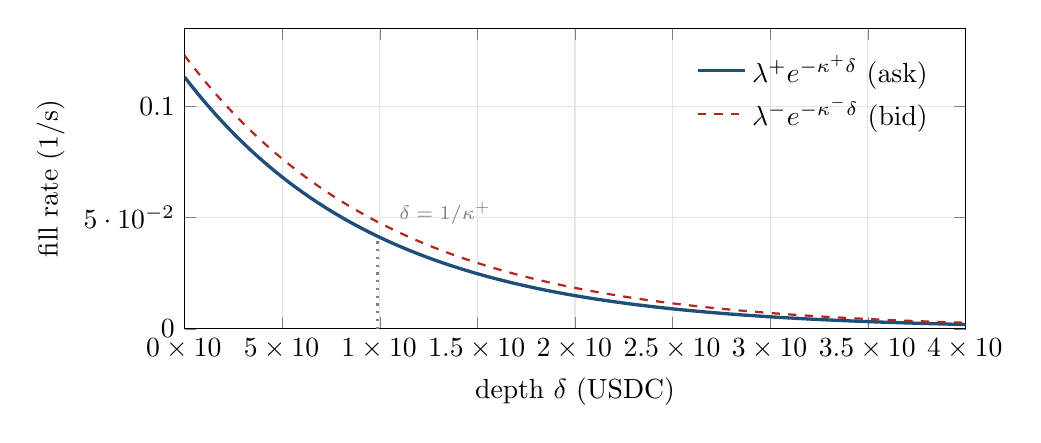
\begin{tikzpicture}
\begin{axis}[
  width=11.5cm, height=5.4cm,
  xlabel={depth $\delta$ (USDC)},
  ylabel={fill rate (1/s)},
  xmin=0, xmax=4e-4, ymin=0,
  grid=major, grid style={gray!20},
  legend style={draw=none, fill=none, at={(0.97,0.95)}, anchor=north east},
  scaled x ticks=false,
  xticklabel style={/pgf/number format/sci, /pgf/number format/sci generic={mantissa sep=,exponent={\times10^{#1}}}},
]
\addplot[NavyLink, very thick, domain=0:4e-4, samples=120]
  {0.11312967808603971*exp(-10123.135078777144*x)};
\addlegendentry{$\lambda^{+}e^{-\kappa^{+}\delta}$ (ask)}
\addplot[BoxTrap, thick, dashed, domain=0:4e-4, samples=120]
  {0.12276729961791137*exp(-9484.501217326813*x)};
\addlegendentry{$\lambda^{-}e^{-\kappa^{-}\delta}$ (bid)}
\addplot[gray, dotted, thick] coordinates {(9.8784e-5,0) (9.8784e-5,0.0416)};
\node[gray, anchor=west, font=\scriptsize] at (axis cs:1.05e-4,0.052) {$\delta=1/\kappa^{+}$};
\end{axis}
\end{tikzpicture}
\caption{Fill rate against depth at the live CASHCAT calibration. At
$\delta = 1/\kappa$ the rate has fallen to $\lambda/e$.}
\end{figure}

\subsection{How the mid-price moves: adverse selection}

This is what distinguishes \S10.4.1 from the simpler market-making models earlier
in the chapter. The mid-price is not a pure random walk; it \emph{jumps} when a
market order arrives, in the direction of that order:
\begin{equation}
  dS_t \;=\; \sigma\, dW_t \;+\; \varepsilon^{+} dM^{+}_t \;-\; \varepsilon^{-} dM^{-}_t,
  \tag{10.22}
  \label{eq:1022}
\end{equation}
where $M^{\pm}$ count buy and sell market orders, and the jump sizes
$\varepsilon^{\pm}$ are i.i.d.\ draws with means $\epsb^{\pm} =
\mathbb{E}[\varepsilon^{\pm}]$.

\begin{intuition}
Read \eqref{eq:fillrate} and \eqref{eq:1022} together and the problem is
obvious. A buy market order is exactly the event that (a) fills our ask and
(b) pushes the mid up by $\varepsilon^{+}$. We sell, and then the price rises.
Being filled is itself bad news. The model's answer is to quote $\epsb^{+}$
further out so the average fill is compensated for the average subsequent move.
\end{intuition}

\subsection{Inventory and cash}

Each fill moves inventory by exactly one unit. The book's (10.2) states this as
$Q_t = N^{-}_t - N^{+}_t$; in differential form, which is how it is usually
quoted,
\begin{equation}
  dQ_t \;=\; dN^{-}_t - dN^{+}_t,
  \tag{cf.\ 10.2}
\end{equation}
where $N^{-}$ counts our filled bids and $N^{+}$ our filled asks. Note this is a
\emph{unit-jump} process: $q$ is an integer, and the whole model is defined only
on integers. That assumption returns to bite in \S\ref{sec:reading}.

Cash accrues at the quoted price on each fill, and the position is bounded to
$\underline{q} \le q \le \bar{q}$ -- at the boundary the model simply stops
quoting the side that would push it further out.

\subsection{What the agent is trying to maximise}

The performance criterion (p.~262) is
\begin{equation}
  H^{\delta}(t,x,S,q) \;=\;
  \mathbb{E}_{t,x,S,q}\!\left[
    X^{\delta}_T + Q^{\delta}_T\bigl(S_T - \alpha Q^{\delta}_T\bigr)
    - \phi\!\int_t^T \bigl(Q^{\delta}_u\bigr)^2 du
  \right],
  \label{eq:criterion}
\end{equation}
and the value function is $H = \sup_{\dpm} H^{\delta}$. Three terms:

\begin{description}[leftmargin=1.4cm,style=nextline]
\item[$X^{\delta}_T$] the cash collected from making markets. The thing we want.
\item[$Q_T(S_T - \alpha Q_T)$] liquidate whatever is left at $T$ at the mid,
  paying a penalty $\alpha Q_T^2$ for the privilege. $\alpha$ prices the cost of
  dumping a position at market.
\item[$-\phi\int (Q_u)^2 du$] a \emph{running} charge for holding inventory at
  all. Every second spent with $q \ne 0$ costs $\phi q^2$.
\end{description}

\begin{intuition}
$\phi$ and $\alpha$ are the two risk dials. $\phi$ says ``I dislike holding
inventory \emph{at any moment}''; $\alpha$ says ``I dislike being caught holding
inventory \emph{at the end}''. Their \emph{ratio} decides whether the strategy
unwinds steadily throughout, or procrastinates and flattens near the deadline.
We return to this in \S\ref{sec:phialpha}, where it turns out our calibration is
overwhelmingly $\phi$-dominated.
\end{intuition}

\subsubsection{Where \texorpdfstring{$\phi$}{phi} comes from: the utility-maximising maker}
\label{sec:utility}

A reasonable objection to \eqref{eq:criterion} is that $\phi\int q^2$ looks
arbitrary. Why penalise inventory quadratically, in a criterion that is otherwise
about expected cash?

The book answers this in \S10.3, ``Utility Maximising Market Maker''. Suppose
instead the agent has no running penalty at all, and simply maximises the
expected \emph{exponential utility} $u(x) = -e^{-\gamma x}$ of terminal wealth,
with risk aversion $\gamma$. Working through the corresponding equation gives
optimal depths
\[
  \delta^{*,\pm} \;=\; \frac{1}{\gamma}\log\!\left(1 + \frac{\gamma}{\kappa^{\pm}}\right)
  + g(t,q) - g(t,q\mp1),
  \tag{10.19}
\]
which is the same shape as the running-penalty answer, with $1/\kappa^{\pm}$
replaced by $\hat{\kappa}^{\pm-1} = \gamma^{-1}\log(1+\gamma/\kappa^{\pm})$ ---
a risk-aversion bias that vanishes as $\gamma \downarrow 0$. Matching the two
problems term by term, the book finds they are the \emph{same problem} under
\begin{equation}
  \boxed{\;\phi = \tfrac{1}{2}\sigma^{2}\gamma,
  \qquad \lambda_0 = e^{+1}\hat{\lambda},
  \qquad \kappa_0 = \kappa\;}
  \label{eq:phigamma}
\end{equation}
(an unnumbered display on p.~261; the consequences are its eqs.~10.20 and 10.21).
With that re-scaling the optimal strategies differ only by the constant
$(\hat{\kappa}^{\pm})^{-1} - (\kappa_0^{\pm})^{-1}$, and the value functions are
related by $H = -\gamma^{-1}\log(-G)$.

\begin{intuition}
This is worth pausing on. The running penalty is not a hack -- it is
\emph{equivalent} to honest risk aversion, and the exchange rate between them is
$\phi = \tfrac12\sigma^2\gamma$. In particular $\phi$ should be
\textbf{proportional to variance}: the same risk aversion in a more volatile
market implies a larger inventory penalty. That is exactly what the code's
volatility channel does (\S\ref{sec:phicode}), and \eqref{eq:phigamma} is its
justification.
\end{intuition}

\begin{departure}
Two honest caveats on borrowing this result. First, the book proves it for the
\emph{base} model of \S10.2, which has no adverse-selection jumps --- there
$\sigma$ is the whole of the price movement, whereas in \S10.4.1 part of the
variance is the $\varepsilon^{\pm}$ jumps. Second, and for the same reason, the
$\sigma^{2}$ we measure is the \emph{total} mid variance including those jumps,
so the volatility channel mildly double-counts adverse selection. At the live
calibration that channel is about 6\% of $\phi$, so the effect is small --- but
it is there, and \eqref{eq:phigamma} is a motivation for the term rather than a
derivation of it.
\end{departure}

\subsection{Reducing the problem}

The value function $H$ depends on four variables, which is three too many. The
book's ansatz strips out cash and price:
\begin{equation}
  H(t,x,S,q) \;=\; x + qS + h(t,q).
  \tag{10.25}
\end{equation}
Cash is worth its face value, the inventory is worth the mid, and everything
interesting -- the option value of being a market maker with $q$ units in hand --
is in $h(t,q)$, a function of \emph{time and an integer}.

Substituting this into the dynamic programming equation --- the book's (10.23),
which we do not reproduce because nothing downstream reads it directly --- makes
the $x$ and $S$ dependence cancel, collapsing four variables to two:
\begin{equation}
\begin{aligned}
  \phi q^{2} \;=\; \partial_t h
  &+ \lambda^{+}\sup_{\dplus}\Bigl\{ e^{-\kappa^{+}\dplus}
      \bigl(\dplus - \epsb^{+} + h_{q-1} - h_q\bigr)\Bigr\}\mathbf{1}_{q>\underline{q}}\\
  &+ \lambda^{-}\sup_{\dminus}\Bigl\{ e^{-\kappa^{-}\dminus}
      \bigl(\dminus - \epsb^{-} + h_{q+1} - h_q\bigr)\Bigr\}\mathbf{1}_{q<\bar{q}}\\
  &+ \bigl(\epsb^{+}\lambda^{+} - \epsb^{-}\lambda^{-}\bigr) q,
\end{aligned}
  \tag{10.26}
  \label{eq:1026}
\end{equation}
subject to the terminal condition $h(T,q) = -\alpha q^{2}$. Here and below
$h_q$ is shorthand for $h(t,q)$ at the current time.

\begin{intuition}
Read the two $\sup$ terms as ``rate of fills $\times$ profit per fill''. The
profit per fill on the ask is: the depth you collect ($\dplus$), minus what
adverse selection costs you ($\epsb^{+}$), plus the change in your position's
option value from going one unit shorter ($h_{q-1}-h_q$). Choosing $\dplus$
trades the rate against the profit, and $\sup$ picks the best point.

The last line is a \emph{drift}: even a maker who never trades is exposed,
because market orders move the mid and we hold $q$ of the asset. It is small but
it is not zero, and it is easy to drop by accident.
\end{intuition}

\subsection{The optimal depths}

Each $\sup$ in \eqref{eq:1026} is one-dimensional and has a closed form. Writing
$\Delta h = h_{q\mp1} - h_q$ for the relevant side, maximise
$f(\delta) = e^{-\kappa\delta}(\delta - \epsb + \Delta h)$:
\[
  f'(\delta) = e^{-\kappa\delta}\Bigl[1 - \kappa\bigl(\delta - \epsb + \Delta h\bigr)\Bigr] = 0
  \;\Longrightarrow\;
  \delta^{*} = \frac{1}{\kappa} + \epsb - \Delta h .
\]
That is the whole derivation. Written out for both sides:
\begin{equation}
\boxed{
\begin{aligned}
  \dplus{}^{,*}(t,q) &= \frac{1}{\kappa^{+}} + \epsb^{+} - h(t,q-1) + h(t,q),
    &&q \ne \underline{q},\\[2pt]
  \dminus{}^{,*}(t,q) &= \frac{1}{\kappa^{-}} + \epsb^{-} - h(t,q+1) + h(t,q),
    &&q \ne \bar{q}.
\end{aligned}}
  \tag{10.27}
  \label{eq:1027}
\end{equation}

Substituting $\delta^*$ back gives the value of the $\sup$, which we will need in
a moment:
\begin{equation}
  \lambda\, e^{-\kappa\delta^{*}}\bigl(\delta^{*} - \epsb + \Delta h\bigr)
  \;=\; \frac{\lambda}{\kappa}\, e^{-\kappa\delta^{*}} .
  \label{eq:supvalue}
\end{equation}

\begin{intuition}
The three terms of (10.27) are the three ideas of this document:
\begin{enumerate}[nosep]
  \item $1/\kappa^{\pm}$ --- \textbf{rent}. How much you can charge before fills
    dry up. Set purely by liquidity.
  \item $\epsb^{\pm}$ --- \textbf{adverse-selection recovery}. Step back by the
    average post-fill move, so the average fill breaks even against it.
  \item $h(t,q) - h(t,q\mp1)$ --- \textbf{inventory pressure}. The only term
    that knows what you are holding. This is what skews the quotes.
\end{enumerate}
The exclusions $q\ne\underline{q}$, $q\ne\bar{q}$ mean: at the top of the
inventory band there is \emph{no bid at all}, and at the bottom there is no ask.
\end{intuition}

\subsection{Solving for \texorpdfstring{$h$}{h}}

Equation \eqref{eq:1026} is still non-linear because of the exponentials, but
when $\kappa^{+} = \kappa^{-} = \kappa$ it linearises exactly. Substitute
\eqref{eq:supvalue} into \eqref{eq:1026} and set
\[
  h(t,q) = \frac{1}{\kappa}\log \omega(t,q).
\]
Then $e^{-\kappa\delta^{*}} = e^{-1-\kappa\epsb}\,e^{\kappa\Delta h}
= e^{-1-\kappa\epsb}\,\omega_{q\mp1}/\omega_q$, so defining
\[
  \tilde{\lambda}^{\pm} \;=\; \lambda^{\pm} e^{-1-\kappa\epsb^{\pm}}
\]
and, since $h = \kappa^{-1}\log\omega$ gives $\partial_t h =
\partial_t\omega_q / (\kappa\omega_q)$, multiplying \eqref{eq:1026} through by
$\kappa\omega_q$ turns every term linear:
\[
  \partial_t \omega_q
  + \tilde{\lambda}^{+}\omega_{q-1}
  + \tilde{\lambda}^{-}\omega_{q+1}
  + \Bigl[\kappa q\bigl(\lambda^{+}\epsb^{+} - \lambda^{-}\epsb^{-}\bigr) - \phi\kappa q^{2}\Bigr]\omega_q
  \;=\; 0 .
\]
Stacking the $\omega_q$ into a vector, that is $\partial_t\boldsymbol{\omega} +
\mathbf{A}\boldsymbol{\omega} = \mathbf{0}$ with
\begin{equation}
  \mathbf{A}_{i,q} =
  \begin{cases}
    q\kappa\bigl(\epsb^{+}\lambda^{+} - \epsb^{-}\lambda^{-}\bigr) - \phi\kappa q^{2},
      & i = q,\\[2pt]
    \tilde{\lambda}^{+}, & i = q-1,\\[2pt]
    \tilde{\lambda}^{-}, & i = q+1,\\[2pt]
    0, & \text{otherwise.}
  \end{cases}
  \tag{10.28}
  \label{eq:1028}
\end{equation}
The terminal condition $h(T,q) = -\alpha q^2$ becomes $\omega(T,q) = e^{\kappa h}
= e^{-\alpha\kappa q^{2}}$, and a linear ODE with a constant matrix has one
answer:
\begin{equation}
  \boldsymbol{\omega}(t) \;=\; e^{\mathbf{A}(T-t)}\mathbf{z},
  \qquad z_j = e^{-\alpha\kappa j^{2}} .
  \tag{10.29}
\end{equation}

\begin{trap}
\label{trap:kappa}
Look at where $\kappa$ appears in (10.28) and in $z_j = e^{-\alpha\kappa j^2}$:
the model responds to the \emph{products} $\phi\kappa$ and $\alpha\kappa$, never
to $\phi$ or $\alpha$ alone. So \textbf{$\phi$ and $\alpha$ are not
$\kappa$-invariant}. A $\phi$ tuned on one asset means something completely
different on another whose $\kappa$ differs by a factor of ten. This is why the
code tunes the dimensionless $\phi\kappa T$ and $\alpha\kappa$ instead, and
derives $\phi$ and $\alpha$ from them (\S\ref{sec:phicode}).
\end{trap}

% ===========================================================================
\section{Stage 1: estimating the parameters from L2 tick data}
\label{sec:estimation}

The model takes $\kappa^{\pm}, \lambda^{\pm}, \epsb^{\pm}$ (and, through
\eqref{eq:phigamma}, $\sigma^2$) as given. Real markets do not hand them over,
so they are fitted continuously from the raw feed.

\subsection{The raw data}

A collector (\code{scripts/hyperliquid\_data\_collector.py}) subscribes to two
Hyperliquid websocket streams and writes them to Parquet shards:

\begin{itemize}[nosep]
  \item \textbf{L2 book / BBO}: an \emph{L2} feed reports the order book
    aggregated by price level --- how much is resting at each price --- rather
    than order by order. \emph{BBO} is the ``best bid and offer'', i.e.\ just the
    top level of each side. Each update is written as two rows (one \code{bid},
    one \code{ask}) with price, size, local receive time and exchange time. This
    is the tick data everything else is measured against.
  \item \textbf{Trades}: every public print --- a record that a trade happened
    --- with side and size.
\end{itemize}

Both are loaded once per estimation cycle by
\code{estimator\_common.load\_market\_window()}, which does the unglamorous work
that decides whether the estimates mean anything:

\begin{itemize}[nosep]
  \item \textbf{One clock.} Exchange timestamps are used only if \emph{every}
    stream has $\ge99\%$ coverage of them; otherwise everything falls back to
    local receive time. Never a mixture.
  \item \textbf{A mid series} is built from the dense BBO stream, forward-filled,
    keeping only rows with $0 < \text{bid} < \text{ask}$.
  \item \textbf{Trade de-duplication} on trade id. This is not paranoia: on
    2026-08-16 two collectors sharing one output directory wrote every tick
    twice, silently doubling $\lambda^{\pm}$.
  \item \textbf{Market-order aggregation.} Prints sharing a timestamp and side
    collapse into one market order, taking the \emph{deepest} price. This is what
    makes $\lambda$ ``market orders per second'' rather than ``prints per
    second'', and it is what makes the depth below a \emph{walk} distance.
\end{itemize}

For each market order, the mid \emph{strictly before} it is attached
(\code{merge\_asof(..., allow\_exact\_matches=False)}), and the walk depth is
measured from that mid:
\[
  \text{depth}^{+} = \text{(highest buy print)} - \text{pre-mid},
  \qquad
  \text{depth}^{-} = \text{pre-mid} - \text{(lowest sell print)} .
\]

\begin{intuition}
Depth is measured \textbf{from the mid}, not from the touch. That is deliberate:
it is the same coordinate the strategy quotes in, so a fitted $\kappa$ can be
fed straight back into $\delta$ without a change of variable.
\end{intuition}

\subsection{\texorpdfstring{$\kappa^{\pm}$}{kappa}: how fast fills die off with depth}

Here is the key insight, and it is prettier than it first looks. Our order
resting at depth $\delta$ is filled by a market order exactly when that order
\emph{walks at least as deep as $\delta$}. So
\[
  \text{fill rate}(\delta) \;=\; \Lambda\cdot\Pr[\text{depth} \ge \delta]
  \;=\; \Lambda\cdot S(\delta),
\]
and the model's assumption \eqref{eq:fillrate} is precisely the claim that the
\textbf{survival function} $S(\delta)$ of market-order walk depths is
exponential. Take logs and it is a straight line:
\[
  \log S(\delta) \;=\; c - \kappa\delta .
\]
So $\kappa$ is the slope of a log-survival plot -- no binning, no fill
simulation, just the empirical distribution of how deep market orders reach.

\begin{booktocode}{assumption: $\text{fill rate}(\delta) = \lambda^{\pm}e^{-\kappa^{\pm}\delta}$}
The book takes $\kappa^{\pm}$ as given and never says where it comes from. Our
reading is that the assumption is equivalent to ``market-order walk depths are
exponentially distributed'', which \emph{is} something we can measure directly.
\wecode
A weighted log-linear regression of the empirical survival function
$\log S(\delta) = c - \kappa\delta$, weighted by $\sqrt{\text{tail count}}$:
\end{booktocode}

% SNIPPET: scripts/estimator_common.py:481-504
\begin{lstlisting}
    sorted_depths = np.sort(depths)

    grid = np.unique(sorted_depths[sorted_depths <= support_cap])
    if len(grid) < 3:
        return empty

    # Tail counts via searchsorted: count of depths >= delta.
    tail_counts = n_total - np.searchsorted(sorted_depths, grid, side="left")
    survival = tail_counts.astype(float) / float(n_total)
    mask = (survival > 0) & (tail_counts >= 2)
    grid = grid[mask]
    survival = survival[mask]
    tail_counts = tail_counts[mask]
    if len(grid) < 3:
        return empty

    y = np.log(survival)
    weights = np.sqrt(tail_counts.astype(float))
    design = np.column_stack((np.ones_like(grid), -grid))
    try:
        coef, _, _, _ = np.linalg.lstsq(design * weights[:, None], y * weights, rcond=None)
    except np.linalg.LinAlgError:
        return empty
    intercept, kappa = float(coef[0]), float(coef[1])
\end{lstlisting}

The weights are $\sqrt{\text{tail count}}$, because a survival estimate based on
two observations in the tail is far less precise than one based on two hundred.
Support is capped at the 99th percentile so a single freak sweep cannot lever the
slope.

\begin{trap}
A \textbf{buy} market order lifts the \textbf{ask}, so buy-side depths calibrate
$\kappa^{+}$ -- the parameter that prices \emph{our ask}. Getting this backwards
produces a strategy that skews the wrong way and is very hard to spot.
\end{trap}

\subsection{\texorpdfstring{$\lambda^{\pm}$}{lambda}: how often market orders arrive}

Much simpler: count them and divide by the time actually covered.

% SNIPPET: scripts/get_kappa.py:186-192
\begin{lstlisting}
        data_start_ms = max(window.window_start_ms or 0.0, float(window.mids["ts_ms"].min()))
        covered_seconds = max(((window.window_end_ms or 0.0) - data_start_ms) / 1000.0, 1e-6)

    lambda_plus_raw = n_buy_mos / covered_seconds if covered_seconds > 0 else float("nan")
    lambda_minus_raw = n_sell_mos / covered_seconds if covered_seconds > 0 else float("nan")
    kappa_plus_raw = buy_fit["kappa"]
    kappa_minus_raw = sell_fit["kappa"]
\end{lstlisting}

The coverage window starts at the \emph{later} of the requested start and the
first observed mid, so a cold start with a partially filled window does not
deflate $\lambda$.

\subsection{\texorpdfstring{$\epsb^{\pm}$}{epsilon-bar}: the adverse-selection cost}

$\epsb^{\pm}$ is the average amount the mid moves right after a market order --- a
\emph{markout}, i.e.\ the price change measured a fixed interval after an event.
It is measured over a $200$~ms window:

% SNIPPET: scripts/get_epsilon.py:152-160
\begin{lstlisting}
    post = pd.merge_asof(
        frame,
        mids[['ts_ms', 'mid']].sort_values('ts_ms').rename(columns={'ts_ms': 'mid_ts_ms', 'mid': 'post_mid'}),
        left_on='target_ms',
        right_on='mid_ts_ms',
        direction='backward',
        allow_exact_matches=True,
    )
    post = post.dropna(subset=['post_mid'])
\end{lstlisting}

The result is 3$\sigma$-clipped and floored at zero (the model requires
$\epsb \ge 0$). Events too close to the end of the window are dropped, so the
horizon never runs off the end of the data and biases the mean downwards.

\begin{intuition}
Why 200~ms and not 5~s? Because \eqref{eq:1022} defines $\varepsilon$ as the
jump \emph{at arrival}. A 5-second markout sweeps up every \emph{other} market
order that arrived in between, and those are already accounted for by the drift
term $q(\lambda^{+}\epsb^{+}-\lambda^{-}\epsb^{-})$ in \eqref{eq:1026}. Using a
long markout here would count the same effect twice. The 1\,s and 5\,s markouts
are computed anyway, but only as diagnostics.
\end{intuition}

\subsection{\texorpdfstring{$\sigma^{2}$}{sigma squared}: the variance rate}

Variance of one-second mid increments, per second:

% SNIPPET: scripts/estimator_common.py:551-557
\begin{lstlisting}
    sampled = np.where(fresh, mid[np.clip(idx, 0, None)], np.nan)

    diffs = np.diff(sampled)
    diffs = diffs[np.isfinite(diffs)]
    if len(diffs) < min_samples:
        return None
    sigma2 = float(np.var(diffs)) / step
\end{lstlisting}

The \code{fresh} mask is the interesting part: grid points whose most recent
observation is more than 5 seconds stale are voided rather than forward-filled.
Without it, a collector outage would appear as a single enormous price jump and
read as a volatility spike -- which, through \eqref{eq:phigamma}, would widen
every quote in response to a \emph{data} problem.

\subsection{Smoothing, gating and transport}

\begin{table}[h]
\centering\small
\begin{tabular}{@{}lll@{}}
\toprule
\textbf{Stage} & \textbf{What} & \textbf{Value} \\
\midrule
Window          & trailing data used per fit    & 120 minutes \\
Cadence         & re-fit interval               & 30 s \\
Smoothing       & time-aware EMA, $\alpha = 1-e^{-\Delta t/\tau}$ & $\tau = 300$ s \\
Transport       & one atomic Redis blob per symbol & \code{mm:params:<SYM>} \\
Max age         & strategy refuses older params & 120 s$^{\dagger}$ \\
\bottomrule
\end{tabular}
\caption{The estimator cadence as deployed. $\dagger$~the strategy's own default
is 90~s; \code{user\_data/config.json} raises it to 120~s, so a reader checking
\code{Market\_Making.py} alone will find the smaller number.}
\end{table}

A cycle that fails its own quality checks ships \emph{raw} values and does not
blend, so one bad window cannot poison the EMA. The strategy then re-checks
everything independently on every single quote: schema version, status,
freshness, $\kappa>0$, $\lambda\ge0$, $\epsb\ge0$, fit quality
($R^2 \ge 0.30$, $\ge 6$ fit points, $\ge 50$ impact events), and a
\textbf{toxicity} gate $\max(\kappa^{+}\epsb^{+}, \kappa^{-}\epsb^{-}) \le 1.5$.

\begin{intuition}
The toxicity number $\kappa\epsb$ is dimensionless and deeply meaningful: it is
adverse-selection cost measured in units of the natural rent $1/\kappa$. If
$\kappa\epsb > 1$, the average fill loses more to the subsequent price move than
the entire monopoly rent is worth, and no amount of clever quoting fixes it. The
live CASHCAT values sit near $0.26$.
\end{intuition}

% ===========================================================================
\section{Stage 2: solving for \texorpdfstring{$h$}{h}}
\label{sec:solving}

\subsection{Choosing \texorpdfstring{$\phi$ and $\alpha$}{phi and alpha}}
\label{sec:phicode}

\begin{booktocode}{$\phi$ and $\alpha$ are free parameters}
The book treats $\phi$ (running penalty) and $\alpha$ (terminal penalty) as
constants the agent chooses, and \S10.3 pins one of them down:
$\phi = \tfrac12\sigma^{2}\gamma$ for an agent with risk aversion $\gamma$.
\wecode
We do \emph{not} configure $\phi$ and $\alpha$ directly, because
Trap~\ref{trap:kappa} shows they are not $\kappa$-invariant. We configure the
dimensionless $\phi\kappa T$ and $\alpha\kappa$ and derive the rest, then add the
volatility term that \S10.3 calls for:
\end{booktocode}

% SNIPPET: scripts/mm_core.py:413-422
\begin{lstlisting}
    if kappa_avg > 0:
        # Derive from the dimensionless targets so the same config expresses the
        # same risk trade-off at any kappa.
        if float(config.hjb_phi_kappa_t) > 0 and horizon > 0:
            phi = float(config.hjb_phi_kappa_t) / (kappa_avg * horizon) + vol_delta
            phi_source = "kappa_relative+sigma2" if vol_delta else "kappa_relative"
            ceiling = float(config.hjb_phi_kappa_t_max)
            if ceiling > 0 and phi * kappa_avg * horizon > ceiling:
                phi = ceiling / (kappa_avg * horizon)
                phi_source += "+capped"
\end{lstlisting}

So the live $\phi$ and $\alpha$ are
\[
  \phi \;=\; \frac{(\phi\kappa T)_{\text{target}}}{\bar{\kappa}T}
             \;+\; \underbrace{\gamma\,\sigma^{2}\,u}_{\text{volatility channel}},
  \qquad
  \alpha \;=\; \frac{(\alpha\kappa)_{\text{target}}}{\bar{\kappa}},
\]
with $\bar\kappa$ the mean of $\kappa^\pm$, $u$ the inventory unit size in base
asset, and $\gamma = 0.05$. The volatility channel is the code's realisation of
\eqref{eq:phigamma}: risk aversion times variance. If $\sigma^2$ is missing the
term is simply dropped -- a quiet volatility feed must never stop the quoter.

\subsection{Choosing the number: what a sweep of \texorpdfstring{$\phi\kappa T$}{phi kappa T} actually shows}
\label{sec:phisweep}

$\phi\kappa T = 10$ is the shipped value. It is worth seeing the evidence,
because the evidence is not what the configuration comment claims.

Replaying the whole pipeline over one pinned 18.67-hour CASHCAT tape
(115{,}364 book updates, 46{,}072 trades), varying only $\phi\kappa T$ and
deliberately running well past the configured ceiling of 50:

\begin{table}[h]
\centering\small
\begin{tabular}{@{}rrrrr@{}}
\toprule
$\phi\kappa T$ & PnL (USDC) & maker fills & USDC per fill & \\
\midrule
  0.05 & $-114.61$ & 1928 & $-0.059$ & \\
  0.20 & $-133.22$ & 1959 & $-0.068$ & \\
  1.00 & $-135.94$ & 1867 & $-0.073$ & worst \\
  3.00 & $-119.40$ & 1686 & $-0.071$ & \\
 10.00 & $-95.95$  & 1405 & $-0.068$ & \textbf{shipped} \\
 20.00 & $-63.58$  & 1121 & $-0.057$ & \\
 50.00 & $-65.09$  &  784 & $-0.083$ & ceiling \\
100.00 & $-57.75$  &  614 & $-0.094$ & \\
200.00 & $-47.14$  &  427 & $-0.110$ & \\
400.00 & $-24.83$  &  338 & $-0.073$ & best tested \\
\bottomrule
\end{tabular}
\caption{Running-penalty sweep, one pinned tape, quote attempts held at
$\approx$60{,}800 throughout. The best setting tested is the largest one tested.}
\label{tab:phisweep}
\end{table}

\begin{figure}[h]
\centering
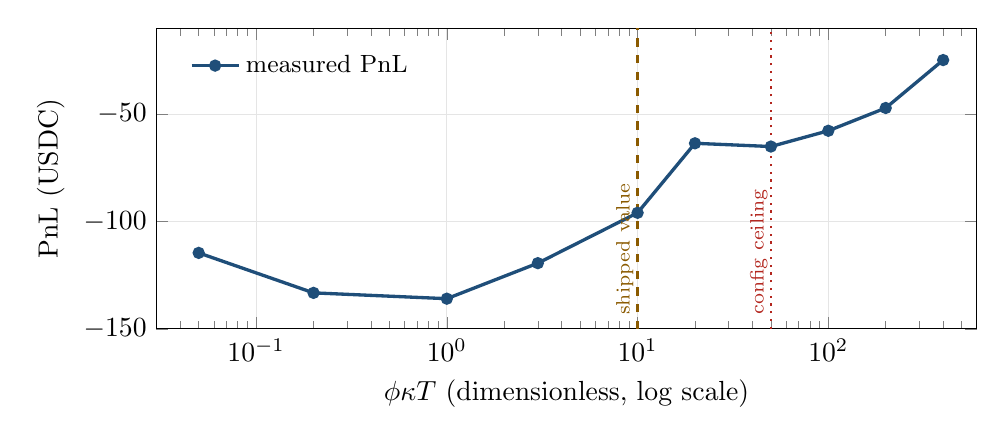
\begin{tikzpicture}
\begin{semilogxaxis}[
  width=12cm, height=5.4cm,
  xlabel={$\phi\kappa T$ (dimensionless, log scale)},
  ylabel={PnL (USDC)},
  grid=major, grid style={gray!20},
  xmin=0.03, xmax=600, ymin=-150, ymax=-10,
  legend style={draw=none, fill=none, at={(0.03,0.95)}, anchor=north west, font=\small},
]
\addplot[NavyLink, very thick, mark=*, mark size=1.6] coordinates {
  (0.05,-114.607) (0.2,-133.224) (1.0,-135.936) (3.0,-119.395)
  (10.0,-95.950) (20.0,-63.581) (50.0,-65.087) (100.0,-57.750)
  (200.0,-47.140) (400.0,-24.825)};
\addlegendentry{measured PnL}
\addplot[BoxDeparture, dashed, thick] coordinates {(10,-150) (10,-10)};
\node[BoxDeparture, anchor=south west, font=\scriptsize, rotate=90]
  at (axis cs:10.7,-148) {shipped value};
\addplot[BoxTrap, dotted, thick] coordinates {(50,-150) (50,-10)};
\node[BoxTrap, anchor=south west, font=\scriptsize, rotate=90]
  at (axis cs:54,-148) {config ceiling};
\end{semilogxaxis}
\end{tikzpicture}
\caption{The same data. Past $\phi\kappa T \approx 1$ the curve improves
monotonically; it never turns back down within a factor of 400.}
\label{fig:phisweep}
\end{figure}

\begin{trap}
The configuration comment in \code{mm\_core.py} records an earlier sweep on a
9.8-hour tape that found ``an inverted U with the optimum at 10--20''. On this
longer tape \textbf{there is no inverted U and no interior optimum}. The loss
shrinks monotonically as the inventory penalty rises, right out to
$\phi\kappa T = 400$ --- eight times the configured ceiling --- where it is the
smallest of the whole sweep.

The honest reading is uncomfortable and worth stating plainly. Look at the
fills column of Table~\ref{tab:phisweep}: 1959 down to 338. Look at USDC per fill: it sits between $-0.06$
and $-0.11$ across a factor of 8000 in the parameter. \textbf{Each fill costs
roughly the same no matter how the model is tuned; all $\phi$ does is change how
many fills you take.} Total loss therefore tracks fill count, not cleverness, and
``turning $\phi$ up'' is not finding a better trade-off --- it is trading less.
The limit of that logic is not quoting at all.

Two consequences. First, do not read $\phi\kappa T = 10$ as a measured optimum;
it is a middling point on a monotone curve, and the evidence originally cited for
it did not replicate. Second, this sweep is not really measuring the inventory
penalty at all --- it is measuring the fact that on this instrument, at this
latency, the marginal maker fill has negative expected value. No setting of
$\phi$ fixes that, which is exactly what \S\ref{sec:departures} item~8 is about.
\end{trap}

\subsection{Building \texorpdfstring{$\mathbf{A}$}{A}}

\begin{booktocode}{eq.~(10.28) and (10.29)}
$\mathbf{A}_{i,q}$ has $q\kappa(\epsb^{+}\lambda^{+}-\epsb^{-}
\lambda^{-}) - \phi\kappa q^{2}$ on the diagonal, $\tilde{\lambda}^{+}$ and
$\tilde{\lambda}^{-}$ off it with $\tilde{\lambda}^{\pm} = \lambda^{\pm}
e^{-1-\kappa\epsb^{\pm}}$; then $\boldsymbol{\omega}(t) = e^{\mathbf{A}(T-t)}
\mathbf{z}$ with $z_j = e^{-\alpha\kappa j^{2}}$.
\wecode
Line for line, with no rearrangement --- compare \eqref{eq:1028}:
\end{booktocode}

% SNIPPET: scripts/hjb.py:227-241
\begin{lstlisting}
    lam_tilde_p = lam_p * np.exp(-1.0 - kappa * eps_p)
    lam_tilde_m = lam_m * np.exp(-1.0 - kappa * eps_m)

    q_grid = np.arange(q_min, q_max + 1)
    d = len(q_grid)
    A = np.zeros((d, d))

    for i, q in enumerate(q_grid):
        A[i, i] = q * kappa * (lam_p * eps_p - lam_m * eps_m) - phi * kappa * (q ** 2)
        if i > 0:
            A[i, i - 1] = lam_tilde_p
        if i < d - 1:
            A[i, i + 1] = lam_tilde_m

    z = np.exp(-alpha * kappa * (q_grid ** 2))
\end{lstlisting}

Every symbol maps directly: \code{lam\_tilde\_p} is $\tilde{\lambda}^{+} =
\lambda^{+}e^{-1-\kappa\epsb^{+}}$, the diagonal is
$q\kappa(\lambda^{+}\epsb^{+}-\lambda^{-}\epsb^{-}) - \phi\kappa q^{2}$, and
\code{z} is $z_j = e^{-\alpha\kappa j^{2}}$.

\begin{trap}
The off-diagonal placement deserves a second look. \code{q\_grid} is
\emph{ascending}, while the book stacks $\boldsymbol{\omega}$ \emph{descending}
from $\bar{q}$ down to $\underline{q}$, and the book's case list does not say
which index of $\mathbf{A}_{i,q}$ is the row. Do not try to read it off; derive
it. The derivation in \S\ref{sec:model} gives the row at inventory $q$ the term
$\tilde{\lambda}^{+}\omega_{q-1}$, because a \textbf{buy} MO (rate $\lambda^{+}$)
fills our ask and takes $q \to q-1$. That is exactly
\code{A[i, i-1] = lam\_tilde\_p}. The code is right.
\end{trap}

\subsection{Two solvers}

\paragraph{Closed form, when $\kappa^{+} = \kappa^{-}$.} Diagonalise
$\mathbf{A} = V\Lambda V^{-1}$ and (10.29) evaluates in one shot for
every $t$ at once. The implementation carries one wrinkle worth understanding:
computing $e^{\mathbf{A}T}$ directly overflows once an eigenvalue times $T$ grows past
about $709$ in magnitude, returning silent NaNs. Factoring
$e^{\theta} = e^{\theta-m}e^{m}$ with $m = \max_j\theta_j$ and adding $m$ back
after the logarithm is algebraically exact and cannot overflow.

\paragraph{Backward Euler, when $\kappa^{+} \ne \kappa^{-}$.} With different
$\kappa$s the log substitution no longer linearises the problem, so
\eqref{eq:1026} is integrated backwards from $h(T,q) = -\alpha q^{2}$ in
\code{n\_steps} implicit steps, each solved by a damped Newton iteration.

Write \eqref{eq:1026} as $\partial_t h = -G(h)$, so $G$ collects the two $\sup$
terms, the $-\phi q^2$ and the drift. Because $G$ depends on $h$ only through the
neighbour differences $h_{i\pm1} - h_i$, its Jacobian is tridiagonal and known
analytically:
\[
  \frac{\partial G_i}{\partial h_{i-1}} = s^{+},\qquad
  \frac{\partial G_i}{\partial h_{i}} = -s^{+}-s^{-},\qquad
  \frac{\partial G_i}{\partial h_{i+1}} = s^{-},
\]
where $s^{\pm}$ is each side's derivative of its $\sup$ value with respect to
that difference. So each Newton step is a banded solve rather than a dense one. \textbf{This is
the solver the live bot uses}; the closed form is kept as the reference that the
test suite checks it against.

\begin{intuition}
Why is the derivative free? At the optimum, $\text{value} =
(\lambda/\kappa)e^{-\kappa\delta^{*}}$ and $\delta^{*} = 1/\kappa + \epsb -
\Delta h$, so $\partial(\text{value})/\partial(\Delta h) = \kappa \cdot
\text{value}$. The derivative is the function itself times $\kappa$ -- no finite
differences anywhere.
\end{intuition}

\subsection{From \texorpdfstring{$h$}{h} to depths}

\begin{booktocode}{eq.~(10.27)}
$\dplus{}^{,*} = \tfrac{1}{\kappa^{+}} + \epsb^{+} - h(q-1) + h(q)$ for
$q \ne \underline{q}$, and the mirror for the bid at $q \ne \bar{q}$.
\wecode
The subtraction is inside the shared helper \code{\_optimal\_delta\_and\_value},
which returns $\delta^{*} = 1/\kappa + \epsb - \Delta h$. What is left here is
the loop over $q$ and, more importantly, the two indicator functions:
\end{booktocode}

% SNIPPET: scripts/hjb.py:144-158
\begin{lstlisting}
    delta_plus = np.full(d, np.inf, dtype=float)
    delta_minus = np.full(d, np.inf, dtype=float)
    for i in range(d):
        h_q = h_vec[i]
        if i > 0:
            raw_plus, _, _ = _optimal_delta_and_value(
                lam_p, kappa_p, eps_p, h_vec[i - 1] - h_q, clip_at_zero=clip_deltas
            )
            delta_plus[i] = max(0.0, raw_plus) if clip_deltas else raw_plus
        if i < d - 1:
            raw_minus, _, _ = _optimal_delta_and_value(
                lam_m, kappa_m, eps_m, h_vec[i + 1] - h_q, clip_at_zero=clip_deltas
            )
            delta_minus[i] = max(0.0, raw_minus) if clip_deltas else raw_minus
    return delta_plus, delta_minus
\end{lstlisting}

Note how the book's indicator functions $\mathbf{1}_{q>\underline{q}}$,
$\mathbf{1}_{q<\bar{q}}$ are realised: both arrays are \emph{initialised to
$+\infty$}, and a side is only written when its neighbour exists. At
$q = \underline{q}$ the \code{if i > 0} guard is false, so the ask stays infinite.
Infinity here means \textbf{``this side is switched off''}, not ``very deep'' --
a distinction the rest of the pipeline is careful to preserve.

\subsection{A normalisation you must know about}

Both solvers subtract each time slice's own maximum, so that
$\max_q h(t,q) = 0$ on every slice. This is safe because everything downstream
reads only \emph{differences within a slice} -- (10.27) uses
$h_{q\mp1} - h_q$ and nothing else -- and it is \emph{necessary} because in the
steady state the unnormalised $h$ drifts linearly in $t$ until its level swamps
the $O(1/\kappa)$ differences the depths are made of.

\begin{trap}
The consequence: in the returned surface, \textbf{levels are not comparable
across time slices}. Differences within a slice are exact. Do not plot
\code{h\_surface} as if it were a value function; it is a value function plus a
different constant on every row.
\end{trap}

\subsection{What the solution looks like}

\begin{figure}[h]
\centering
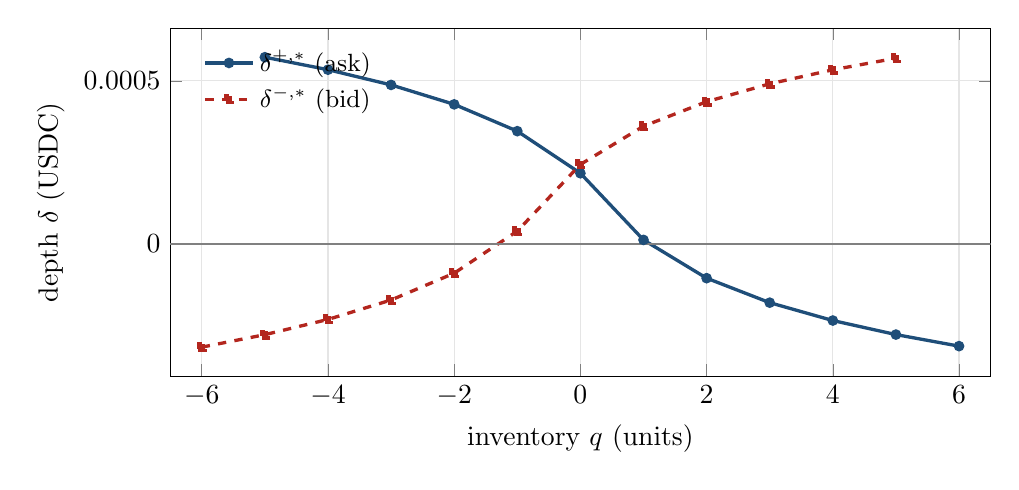
\begin{tikzpicture}
\begin{axis}[
  width=12cm, height=6cm,
  xlabel={inventory $q$ (units)},
  ylabel={depth $\delta$ (USDC)},
  xmin=-6.5, xmax=6.5, xtick={-6,-4,-2,0,2,4,6},
  grid=major, grid style={gray!20},
  legend style={draw=none, fill=none, at={(0.03,0.97)}, anchor=north west, font=\small},
  scaled y ticks=false,
  yticklabel style={/pgf/number format/fixed, /pgf/number format/precision=5},
]
\addplot[NavyLink, very thick, mark=*, mark size=1.3] coordinates {
  (-5,5.72590804e-4) (-4,5.34324665e-4) (-3,4.87696805e-4) (-2,4.28103683e-4)
  (-1,3.45960325e-4) (0,2.16943383e-4) (1,1.25838060e-5) (2,-1.04640487e-4)
  (3,-1.79740208e-4) (4,-2.34530875e-4) (5,-2.77561222e-4) (6,-3.12972442e-4)};
\addlegendentry{$\delta^{+,*}$ (ask)}
\addplot[BoxTrap, very thick, mark=square*, mark size=1.2, dashed] coordinates {
  (-6,-3.16074195e-4) (-5,-2.77808055e-4) (-4,-2.31180196e-4) (-3,-1.71587074e-4)
  (-2,-8.94437157e-5) (-1,3.95732266e-5) (0,2.43932803e-4) (1,3.61157097e-4)
  (2,4.36256817e-4) (3,4.91047485e-4) (4,5.34077832e-4) (5,5.69489052e-4)};
\addlegendentry{$\delta^{-,*}$ (bid)}
\addplot[gray, thin, domain=-6.5:6.5] {0};
\end{axis}
\end{tikzpicture}
\caption{The solved control at the live CASHCAT calibration, $\tau = 130.8$~s.
Long inventory ($q>0$) tightens the ask and widens the bid, pushing the position
back toward zero. The ask is absent at $q=-6$ and the bid at $q=+6$: the
inventory boundary switches the adding side off entirely. Depths below zero
mean the model would like to quote \emph{through} the mid --- see
\S\ref{sec:assembly}.}
\label{fig:skew}
\end{figure}

Figure~\ref{fig:skew} is the model doing its whole job in one picture. The two
curves cross near $q=0$, where the quotes are symmetric. As inventory grows the
ask falls and the bid rises: sell harder, buy more reluctantly.

% ===========================================================================
\section{Stage 3: reading \texorpdfstring{$\delta^{*}(t,q)$}{delta*(t,q)}}
\label{sec:reading}

The solver hands back a surface indexed by time and integer inventory. Two
questions remain before a number comes out: \emph{which time}, and \emph{which
inventory}.

\subsection{What one unit of inventory is}
\label{sec:unit}

Before either question, a quantity that silently scales everything: what does
$q=1$ actually mean in coins?

The book leaves this open --- $q$ is simply ``units'', and $\bar{q}$ bounds it.
Here the unit is derived from the account so that a full inventory band is a
sensible fraction of capital:
\[
  u \;=\; \frac{\text{available capital}\times\text{target utilisation}
                \times\text{target leverage}}{\bar{q}\times S},
\]
which at 1000~USDC, 74\% utilisation, 2$\times$ leverage, $\bar q = 6$ and
$S = 0.0976$ gives $u \approx 2527$~CASHCAT, so a full $\pm6$ band is about
1480~USDC of notional.

\begin{trap}
$u$ is the denominator of $q = \text{position}/u$, so changing it re-labels the
whole inventory axis --- and it also appears in the volatility term
$\gamma\sigma^{2}u$ of $\phi$. Resizing it while holding a position would
therefore move the quotes for two unrelated reasons at once. The strategy only
ever resizes it \textbf{while flat}.
\end{trap}

\subsection{Which time: the episode clock}

The book's control is genuinely time-dependent. It has a deadline $T$, and the
terminal condition $h(T,q) = -\alpha q^2$ shapes everything before it. A
perpetual futures contract has no deadline, which leaves a real modelling
choice:

\begin{itemize}[nosep]
  \item \code{hjb\_time\_mode = "stationary"} --- always read the $t=0$ slice.
    The agent then never approaches $T$, $\alpha$ never binds, and the time axis
    of \eqref{eq:1026} is decorative.
  \item \code{hjb\_time\_mode = "episodic"} (the default) --- run a repeating
    episode clock of length $T$, and read the slice at the real remaining time.
    The episode restarts at $T$, or early once the position returns to flat ---
    but only after at least 25\% of the horizon has elapsed, so inventory that
    crosses zero repeatedly cannot restart the clock on every round trip.
\end{itemize}

\begin{departure}
The book liquidates whatever is left at $T$ at market and pays $\alpha q^{2}$.
Every quote here is \textbf{post-only} --- an exchange flag meaning ``reject this
order outright if it would execute on arrival'', which guarantees we are always
the maker and never the taker. Taking liquidity to flatten would contradict the
rest of the design. The terminal condition therefore acts
through the \emph{depths} alone, and the clock restarts rather than the position
being closed.
\end{departure}

\subsection{Which inventory: the problem with partial fills}

Equation (10.2) is a unit-jump process, so $h$ and $\delta^{*}$ exist only at
integer $q$. Real fills are partial: a resting order for one unit may be filled
for 0.4 of it, leaving a fractional position that the integer grid cannot name.
Rounding it away discards up to half a unit of live risk -- 0.49 units would read
as flat.

The fix is to interpolate between the bracketing integers. \emph{Which} quantity
gets interpolated matters:

\begin{intuition}
Interpolate the \textbf{depths}, not $h$. Since $\delta$ reads a \emph{difference}
of $h$ across adjacent $q$, a piecewise-linear $h$ produces piecewise-%
\emph{constant} depths that jump at the integers -- exactly as coarse as the
rounding it was meant to replace. Interpolating the depths themselves agrees
with the book exactly at every integer and varies smoothly in between.
\end{intuition}

\begin{booktocode}{eq.~(10.2): $dQ_t = dN^{-}_t - dN^{+}_t$}
Inventory moves in unit jumps, so $q$ is an integer and the book's $h(t,q)$ and
$\delta^{*}(t,q)$ are defined \textbf{only} at integers. The book never says what
to do at $q = 2.4$, because in its world that state cannot occur.
\wecode
It occurs constantly, because fills are partial. We blend the depths linearly
between the two bracketing integers --- exact at every integer, an extension of
our own in between. The bracketing helper has two guards that look redundant and
are not:
\end{booktocode}

% SNIPPET: scripts/mm_core.py:464-475
\begin{lstlisting}
    n = len(axis)
    if n == 1 or value <= axis[0]:
        return 0, 0, 0.0
    if value >= axis[-1]:
        return n - 1, n - 1, 0.0
    hi = int(np.searchsorted(axis, value, side="left"))
    if float(axis[hi]) == float(value):
        return hi, hi, 0.0
    lo = hi - 1
    span = float(axis[hi] - axis[lo])
    weight = 0.0 if span <= 0 else (float(value) - float(axis[lo])) / span
    return lo, hi, weight
\end{lstlisting}

\begin{trap}
\code{side="left"} and the exact-node check protect \emph{opposite} boundaries,
and both are needed. Consider a grid $[-3,\dots,3]$, where $\delta^{+}$ is
infinite at $q=-3$ and $\delta^{-}$ is infinite at $q=+3$.
\begin{itemize}[nosep]
  \item At exactly $q=+2$, \code{side="right"} would return the pair $(2,3)$ with
    weight $0$. The blend checks finiteness \emph{before} it checks the weight,
    sees the infinite $q=3$ node, and switches the \textbf{bid off at $q=2$} ---
    an inventory the model quotes perfectly happily.
  \item At exactly $q=-2$, without the exact-node early return you would get the
    pair $(-3,-2)$ with weight $1$, and the infinite $q=-3$ node would switch the
    \textbf{ask off at $q=-2$}.
\end{itemize}
Returning the node twice consults no neighbour at all, so an integer $q$
reproduces the book exactly and only genuinely fractional inventory blends.
\end{trap}

And the blend itself refuses to average away a disabled side:

% SNIPPET: scripts/mm_core.py:492-498
\begin{lstlisting}
    if not np.isfinite(low) or not np.isfinite(high):
        return float("inf")
    if weight <= 0.0:
        return float(low)
    if weight >= 1.0:
        return float(high)
    return float(low) + weight * (float(high) - float(low))
\end{lstlisting}

\begin{departure}
Because \emph{either} infinite endpoint disables the blend, with $\bar{q}=6$ a
bid stops above $q = 5.0$ rather than $q = 5.5$. This is the conservative
direction: a bid resting at $q=5.9$ would permit a jump to $6.9$, past the
boundary the model is defined on.
\end{departure}

\subsection{What the time axis actually does here}
\label{sec:phialpha}

A natural guess is that the strategy should grow \emph{more} aggressive about
flattening as $t \to T$, because that is when the terminal penalty $\alpha q^2$
is about to be charged. It does the reverse, and the reason is worth
understanding rather than filing as a bug.

The running penalty enters as $\phi\kappa T = 10$ and the terminal one as
$\alpha\kappa = 0.05$: a ratio of $200$ to $1$. The running penalty is what
remains to be \emph{paid} over the time left, so it is largest at the start of an
episode and vanishes at the end. It dominates the surface completely, and the
skew therefore collapses as $\tau \to 0$.

\begin{intuition}
This is not a quirk of our calibration --- it is what the book's own figures
show. Figure 10.8 (p.~265) plots exactly this: depth curves for
$q = -2 \dots 3$, fanned wide at $t=0$ and converging into $T$. Its parameters
are $\phi = 0.02$, $\kappa = 100$, $T = 30$, $\alpha = 0.0001$, so
$\phi\kappa T = 60$ against $\alpha\kappa = 0.01$ --- a ratio of $6000$ to $1$,
even more running-dominated than ours. The book is in the same regime, and our
solver reproduces its shape. Treat the table below as a validation, not an
anomaly.
\end{intuition}

\begin{table}[h]
\centering\small
\begin{tabular}{@{}rrr@{}}
\toprule
$\tau$ (s) & $\delta^{+,*}$ at $q=+2$ & $\delta^{-,*}$ at $q=-2$ \\
\midrule
150.0 & $-1.0464\times10^{-4}$ & $-8.9444\times10^{-5}$ \\
100.0 & $-1.0464\times10^{-4}$ & $-8.9437\times10^{-5}$ \\
 50.0 & $-1.0443\times10^{-4}$ & $-8.9156\times10^{-5}$ \\
 10.0 & $-5.6830\times10^{-5}$ & $-3.9855\times10^{-5}$ \\
  1.0 & $+8.6643\times10^{-5}$ & $+9.6637\times10^{-5}$ \\
  0.0 & $+1.0852\times10^{-4}$ & $+1.1740\times10^{-4}$ \\
\bottomrule
\end{tabular}
\caption{Depth against time-to-go. The unwinding pressure is strongest at the
\emph{start} of an episode and relaxes into the terminal, matching the shape of
the book's Figure 10.8 --- which is in the same running-penalty-dominated regime.}
\label{tab:timeaxis}
\end{table}

The last row of Table~\ref{tab:timeaxis} is a useful check on the whole machine. At $\tau = 0$ we have
$h(T,q) = -\alpha q^{2}$ exactly, so the ask half of \eqref{eq:1027} collapses to
a closed form:
\[
  \dplus{}^{,*}(T,q) = \frac{1}{\kappa^{+}} + \epsb^{+} + \alpha(1-2q).
\]
At $q=2$ with the live numbers that is
$9.87835\times10^{-5} + 2.50349\times10^{-5} - 3\times5.10005\times10^{-6}
= 1.085184\times10^{-4}$, against the solver's $1.0851837\times10^{-4}$ --
agreement to seven significant figures.

\begin{departure}
\code{hjb\_alpha\_kappa} was set to $0.05$ at a time when the strategy only ever
read the $t=0$ slice, so $\alpha$ had almost no effect on any quote and the value
carries no evidence. It is now live and remains unswept. Treat it as untuned.
\end{departure}

% ===========================================================================
\section{Stages 4 and 5: from a depth to a resting order}
\label{sec:assembly}

The model's $\delta$ is not yet a price. Four things happen to it.

\subsection{The arithmetic}

\begin{booktocode}{nothing at all}
This is the one stage with no equation behind it. In the book, $\delta^{*}$
\emph{is} the answer: the agent posts at $S \pm \delta^{*}$ and the model is
done. There are no fees, no tick sizes, no minimum spreads and no exchange that
rejects orders.
\wecode
Everything below is ours, and every line of it can override the model:
\end{booktocode}

% SNIPPET: scripts/mm_core.py:271-285
\begin{lstlisting}

    fee_cushion = float(config.maker_fee_rate) * mid
    extra_cushion = float(config.extra_cushion_bps) / 10_000.0 * mid
    delta_pre_clamp = model * float(config.spread_multiplier) + fee_cushion + extra_cushion
    floor = float(config.min_half_spread_bps) / 10_000.0 * mid
    cap = float(config.max_half_spread_bps) / 10_000.0 * mid
    delta_total = min(max(delta_pre_clamp, floor), cap)

    clamped = None
    if delta_pre_clamp < floor:
        clamped = "floor"
    elif delta_pre_clamp > cap:
        clamped = "cap"

    p95 = finite_float_or_none(depth_p95)
\end{lstlisting}

\begin{table}[h]
\centering\small
\begin{tabular}{@{}llr@{}}
\toprule
\textbf{Step} & \textbf{Expression} & \textbf{Default} \\
\midrule
model term    & $\delta_{\text{model}} \times$ \code{spread\_multiplier} & $1.0$ \\
fee cushion   & \code{maker\_fee\_rate} $\times$ mid & $1.5$ bps \\
extra cushion & \code{extra\_cushion\_bps}$/10^4 \times$ mid & $0$ \\
floor         & \code{min\_half\_spread\_bps}$/10^4 \times$ mid & $1.5$ bps \\
cap           & \code{max\_half\_spread\_bps}$/10^4 \times$ mid & $80$ bps \\
\bottomrule
\end{tabular}
\end{table}

Four design choices are encoded here:

\begin{itemize}
  \item \textbf{The fee cushion is one maker fee per side.} A round trip pays two
    fees and collects the cushion twice.
  \item \textbf{The multiplier scales only the model term}, so widening quotes
    defensively never inflates the fee compensation.
  \item \textbf{Defensive widening should use \code{extra\_cushion\_bps}, not the
    floor.} The extra cushion is \emph{additive}: it shifts both sides equally
    and leaves the inventory skew of Figure~\ref{fig:skew} intact. Raising
    \code{min\_half\_spread\_bps} is a \emph{clamp}, and a clamp flattens the
    skew for every $q$ beneath it.
  \item \textbf{A disabled side returns nothing at all.} When $\delta$ is
    infinite the function returns \code{None} rather than clamping, because
    clamping $\infty$ into $[\text{floor},\text{cap}]$ would silently turn ``do
    not quote'' into ``quote at the floor''.
\end{itemize}

\begin{intuition}
Figure~\ref{fig:skew} shows the model asking for \emph{negative} ask depths once
$q \ge 2$. A negative depth means ``cross the mid to get out''. That is a
coherent instruction -- the model wants the inventory gone -- but this strategy
is post-only, so it cannot be obeyed. The floor is what stops it, and the
\code{clamped} flag records that the model was overruled.
\end{intuition}

\subsection{Rounding, safely}

% SNIPPET: scripts/hyperliquid_alo_executor.py:76-93
\begin{lstlisting}
def round_price_for_side(
    *,
    side: str,
    price: float,
    price_tick_size: float | None,
    rounding_policy: str = "maker_safe",
) -> float:
    """Round price without weakening the intended post-only safety property."""
    if price_tick_size is None or float(price_tick_size) <= 0:
        return float(price)
    is_buy = side_is_buy(side)
    if rounding_policy == "maker_safe":
        rounding = ROUND_FLOOR if is_buy else ROUND_CEILING
    elif rounding_policy == "crossing_probe":
        rounding = ROUND_CEILING if is_buy else ROUND_FLOOR
    else:
        raise ValueError(f"unsupported rounding_policy: {rounding_policy}")
    return _round_to_step(float(price), float(price_tick_size), rounding=rounding)
\end{lstlisting}

Bids round \emph{down}, asks round \emph{up} -- always away from the touch, never
toward it, and in \code{Decimal} rather than binary floating point. A bid rounded
one unit in the last place the wrong way can cross the ask and turn a post-only
order into an exchange rejection.

\subsection{The last check before posting}

% SNIPPET: scripts/mm_core.py:314-325
\begin{lstlisting}
    price_f = finite_float_or_none(price)
    bid_f = finite_float_or_none(best_bid)
    ask_f = finite_float_or_none(best_ask)
    if price_f is None or price_f <= 0:
        return False, "invalid_rate"
    if bid_f is None or ask_f is None or bid_f <= 0 or ask_f <= 0 or bid_f >= ask_f:
        return False, "crossed_or_invalid_book"
    if side == "bid" and price_f >= ask_f:
        return False, "bid_crosses_ask"
    if side == "ask" and price_f <= bid_f:
        return False, "ask_crosses_bid"
    return True, "ok"
\end{lstlisting}

The comparisons are non-strict: a bid resting exactly \emph{at} the best ask
would cross, so equality is rejected too. A crossed or otherwise invalid book
fails closed.

\begin{trap}
Which side of the book a Freqtrade ``entry'' corresponds to \emph{depends on the
leg's role}:
\[
  \text{long leg: entry} = \text{bid},\ \text{exit} = \text{ask};
  \qquad
  \text{short leg: entry} = \text{ask},\ \text{exit} = \text{bid}.
\]
The depth and the price sign must flip together. Taking the depth from one side
and the sign from the other quotes on the wrong side of the book, which the
maker-safety check then rejects -- the observed symptom being a short leg whose
every entry is denied.
\end{trap}

% ===========================================================================
\section{A fully worked example}
\label{sec:worked}

Everything below is produced by running the real pricing code, and every number
is re-checked by \code{scripts/verify\_spread\_doc.py}.

\subsection{Inputs}

One coherent estimator cycle from the live CASHCAT dry run, stamped
2026-08-17T16:20:41Z over a 120-minute window.

\begin{table}[h]
\centering\small
\begin{tabular}{@{}llll@{}}
\toprule
$\kappa^{+}$ & $10{,}123.135$ & $\lambda^{+}$ & $0.113130$ \\
$\kappa^{-}$ & $9{,}484.501$  & $\lambda^{-}$ & $0.122767$ \\
$\epsb^{+}$  & $2.5035\times10^{-5}$ & $\sigma^{2}$ & $3.3370\times10^{-9}$ \\
$\epsb^{-}$  & $2.7263\times10^{-5}$ & mid $S$ & $0.105685$ \\
\midrule
$T$ & 150 s & unit size $u$ & $2527.32$ CASHCAT \\
$\bar{q}$ & 6 & tick & $10^{-5}$ \\
$(\phi\kappa T)_{\text{target}}$ & 10 & $(\alpha\kappa)_{\text{target}}$ & 0.05 \\
\bottomrule
\end{tabular}
\end{table}

Inventory is \textbf{6065.6 CASHCAT}, deliberately not a whole number of units --
this is what a partial fill leaves behind, and it is what the interpolation
exists for. Time-to-go is $\tau = 130.79$~s.

\subsection{Step 1 --- the risk parameters}

\begin{table}[h]
\centering\small
\begin{tabular}{@{}llr@{}}
\toprule
\textbf{Quantity} & \textbf{Formula} & \textbf{Value} \\
\midrule
% CHECK: kappa_avg = 9803.8181
$\bar{\kappa}$ & $\tfrac12(\kappa^{+}+\kappa^{-})$ & $9803.8181$ \\
% CHECK: phi_kappa_relative = 6.8001e-06
$\phi_{\kappa\text{-rel}}$ & $10/(\bar{\kappa}T)$ & $6.8001\times10^{-6}$ \\
% CHECK: vol_delta = 4.2168e-07
volatility term & $\gamma\sigma^{2}u$ & $4.2168\times10^{-7}$ \\
% CHECK: phi_effective = 7.2218e-06
$\phi$ & sum of the two & $7.2218\times10^{-6}$ \\
% CHECK: alpha_effective = 5.1001e-06
$\alpha$ & $0.05/\bar{\kappa}$ & $5.1001\times10^{-6}$ \\
% CHECK: phi_source = kappa_relative+sigma2
\code{phi\_source} & --- & \code{kappa\_relative+sigma2} \\
% CHECK: n_steps = 600
\code{n\_steps} & $\lceil T/0.25\rceil$ & $600$ \\
% CHECK: dt = 0.25
$dt$ & $T/\text{\code{n\_steps}}$ & $0.25$ s \\
\bottomrule
\end{tabular}
\end{table}

The volatility channel contributes about 6\% of $\phi$ here, lifting the
dimensionless product from the configured $10$ to
% CHECK: phi_kappa_t_dimensionless = 10.6201
$\phi\bar{\kappa}T = 10.6201$ -- comfortably below the cap of 50.

\subsection{Step 2 --- inventory}

\begin{table}[h]
\centering\small
\begin{tabular}{@{}llr@{}}
\toprule
% CHECK: q_exact = 2.4
$q_{\text{exact}}$ & $6065.6 / 2527.32$ & $2.4$ \\
% CHECK: q_int = 2
$q$ (integer, for routing) & $\text{round}(q_{\text{exact}})$ & $2$ \\
% CHECK: q_residual = 0.4
$q_{\text{residual}}$ & $q_{\text{exact}} - q$ & $0.4$ \\
\bottomrule
\end{tabular}
\end{table}

That residual of $0.4$ units is roughly $1010$ CASHCAT of live exposure that the
integer grid cannot represent. It is logged on every quote, and a run whose mean
$|q_{\text{residual}}|$ exceeds $0.35$ fails the dry-run quality gate.

\subsection{Step 3 --- reading the depths}

The fractional inventory sits between the $q=2$ and $q=3$ nodes, so each depth is
a blend with weight $0.4$:

\begin{table}[h]
\centering\small
\begin{tabular}{@{}lrrr@{}}
\toprule
& \textbf{at $q=2$} & \textbf{at $q=3$} & \textbf{blended at $q=2.4$} \\
\midrule
% CHECK: delta_plus_q2 = -1.0464e-04
% CHECK: delta_plus_q3 = -1.7974e-04
% CHECK: ask_delta_model = -1.3468e-04
$\delta^{+,*}$ (ask) & $-1.0464\times10^{-4}$ & $-1.7974\times10^{-4}$ & $-1.3468\times10^{-4}$ \\
% CHECK: delta_minus_q2 = 4.3626e-04
% CHECK: delta_minus_q3 = 4.9105e-04
% CHECK: bid_delta_model = 4.5817e-04
$\delta^{-,*}$ (bid) & $4.3626\times10^{-4}$ & $4.9105\times10^{-4}$ & $4.5817\times10^{-4}$ \\
\bottomrule
\end{tabular}
\end{table}

Check the ask by hand: $-1.0464\times10^{-4} + 0.4\times(-1.7974 + 1.0464)\times
10^{-4} = -1.3468\times10^{-4}$. Note it is \textbf{negative}: holding 2.4 units
long, the model wants to sell badly enough to cross the mid.

\subsection{Step 4 --- assembling both prices}

\begin{table}[h]
\centering\small
\begin{tabular}{@{}lrr@{}}
\toprule
& \textbf{bid} & \textbf{ask} \\
\midrule
% CHECK: bid_delta_model = 4.5817e-04
% CHECK: ask_delta_model = -1.3468e-04
model depth $\delta_{\text{model}}$ & $4.5817\times10^{-4}$ & $-1.3468\times10^{-4}$ \\
% CHECK: bid_fee_cushion = 1.5853e-05
% CHECK: ask_fee_cushion = 1.5853e-05
$+$ fee cushion & $1.5853\times10^{-5}$ & $1.5853\times10^{-5}$ \\
% CHECK: bid_delta_pre_clamp = 4.7403e-04
% CHECK: ask_delta_pre_clamp = -1.1883e-04
$=$ pre-clamp & $4.7403\times10^{-4}$ & $-1.1883\times10^{-4}$ \\
\midrule
% CHECK: floor_price = 1.5853e-05
floor ($1.5$ bps) & \multicolumn{2}{c}{$1.5853\times10^{-5}$} \\
% CHECK: cap_price = 8.4548e-04
cap ($80$ bps) & \multicolumn{2}{c}{$8.4548\times10^{-4}$} \\
% CHECK: bid_clamped = None
% CHECK: ask_clamped = floor
clamped? & no & \textbf{yes, at the floor} \\
\midrule
% CHECK: bid_delta_total = 4.7403e-04
% CHECK: ask_delta_total = 1.5853e-05
final $\delta_{\text{total}}$ & $4.7403\times10^{-4}$ & $1.5853\times10^{-5}$ \\
% CHECK: bid_bps = 44.8527
% CHECK: ask_bps = 1.5000
in bps of mid & $44.85$ & $1.50$ \\
\midrule
% CHECK: bid_raw_price = 0.10521097
% CHECK: ask_raw_price = 0.10570085
raw price ($S \mp \delta$) & $0.10521097$ & $0.10570085$ \\
% CHECK: bid_price = 0.10521
% CHECK: ask_price = 0.10571
rounded to tick & $0.10521$ (down) & $0.10571$ (up) \\
\bottomrule
\end{tabular}
\end{table}

\subsection{Reading the result}

% CHECK: quoted_spread_bps = 47.3104
The final quote is wildly asymmetric: the ask sits $1.50$ bps from the mid and
the bid $44.85$ bps away. Those sum to $46.35$ bps, while the quoted spread
measured between the two \emph{rounded} prices is $47.31$ bps --- the extra
$0.96$ bps is tick rounding pushing both prices away from the touch, which at a
$10^{-5}$ tick on a $0.1057$ mid is worth about half a basis point per side.

None of that is a malfunction; the asymmetry is the entire point. Holding 2.4
units long, the strategy is almost giving the inventory away on the ask while
making itself very hard to hit on the bid.

Two diagnostics fire on this quote and both are worth attention:

\begin{itemize}
  \item \textbf{The ask was clamped at the floor.} The model asked for a negative
    depth and got $1.5$ bps instead. The strategy is therefore \emph{not}
    following the model at this inventory --- it is following the constraint. If
    this fires often, the model is telling you the inventory band is too wide for
    the liquidity available.
  \item \textbf{The bid is outside the calibrated range.}
% CHECK: bid_outside_calibrated = True
    At $4.74\times10^{-4}$ it sits beyond the 95th percentile of observed
    market-order walk depths ($3.42\times10^{-4}$). Equation~\eqref{eq:fillrate}
    is being extrapolated past the data that fitted it, so the true fill
    probability there is anybody's guess.
\end{itemize}

% ===========================================================================
\section{Where this departs from the book}
\label{sec:departures}

A faithful implementation is the goal, so the gaps are listed rather than
glossed.

\begin{enumerate}
  \item \textbf{Two instances, one signed inventory.} The book models a single
    agent holding a signed $q$. Freqtrade rests at most one order per pair, so
    two instances on separate sub-accounts present the two sides and a routing
    rule decides which leg owns which side. Net inventory is shared over Redis
    and is what prices both legs, but the decomposition is an approximation.
  \item \textbf{No forced liquidation at $T$}, as described in
    \S\ref{sec:reading}.
  \item \textbf{Fractional inventory is interpolated} over a domain the book does
    not define. Exact at every integer $q$; an extension in between.
  \item \textbf{The fee cushion and the bps clamps} are outside the model
    entirely. The clamps in particular \emph{override} the model whenever it asks
    for a depth below the floor, which the worked example shows is not rare.
  \item \textbf{Leverage and margin} do not appear in the model at all.
  \item \textbf{Perpetual funding} is not in the model either. The replay harness
    can charge it; the control never sees it.
  \item \textbf{Parameters are re-estimated every 30 seconds} and the problem
    re-solved. The agent therefore follows a \emph{sequence} of solutions to
    slightly different problems, not one solution to a fixed problem.
  \item \textbf{The quote is held stale between cycles.} The model assumes
    continuous requoting; the measured median requote interval here is about
    30 seconds. This is the largest practical gap between the theory and the
    deployment, and it is why the project README warns that the stack needs
    co-located infrastructure to be taken seriously.
\end{enumerate}

\begin{intuition}
Item 8 deserves emphasis because it interacts with \S\ref{sec:estimation}.
Adverse selection roughly \emph{doubles} between a 200~ms and a 5~s markout on
this instrument. The model prices $\epsb$ at the 200~ms horizon because that is
what \eqref{eq:1022} means -- but a quote exposed for 30 seconds is selected
against on a far longer horizon than the one it was priced for.
\end{intuition}

Not a departure, despite appearances: the \textbf{volatility term in $\phi$}.
$\S$10.4.1 treats $\phi$ as a constant, but \S10.3 derives
$\phi = \tfrac12\sigma^{2}\gamma$ (\S\ref{sec:utility}), so a $\phi$ that scales
with variance is the book's own correspondence rather than an outside graft. The
code's constant differs ($\gamma\sigma^{2}u$ rather than $\tfrac12\sigma^{2}
\gamma$, with the unit size folded in to match $h$'s per-unit normalisation), so
$\gamma_{\text{inventory-risk}}$ is a knob of its own, not literally the book's
risk aversion.

% ===========================================================================
\appendix
\section{File map}

\begin{table}[h]
\centering\small
\begin{tabular}{@{}ll@{}}
\toprule
\textbf{File} & \textbf{Role} \\
\midrule
\code{scripts/hyperliquid\_data\_collector.py} & L2 book and trade capture to Parquet \\
\code{scripts/estimator\_common.py} & window loading, $\kappa$, $\sigma^2$, EMA \\
\code{scripts/get\_kappa.py} & $\kappa^{\pm}$, $\lambda^{\pm}$, $\sigma^2$ driver \\
\code{scripts/get\_epsilon.py} & $\epsb^{\pm}$ driver \\
\code{scripts/hjb.py} & the two solvers, (10.26)--(10.29) \\
\code{scripts/mm\_core.py} & $\phi$/$\alpha$ scaling, depth lookup, quote assembly \\
\code{scripts/param\_store.py} & Redis transport for the parameter snapshot \\
\code{user\_data/strategies/Market\_Making.py} & the Freqtrade strategy \\
\code{scripts/replay\_market\_maker.py} & offline replay of the whole pipeline \\
\code{scripts/verify\_spread\_doc.py} & checks this document against the code \\
\bottomrule
\end{tabular}
\end{table}

\section{Rebuilding this document}

\begin{lstlisting}[language=bash]
cd docs
latexmk -pdf spread_calculation.tex
python ../scripts/verify_spread_doc.py
\end{lstlisting}

The verifier re-reads every source range quoted above and re-runs the pricing
code to regenerate every number in \S\ref{sec:worked}. If a refactor moves a
function or a default changes, it fails.

\section{Further reading}

Cartea, \'A., Jaimungal, S. and Penalva, J. (2015). \emph{Algorithmic and
High-Frequency Trading}. Cambridge University Press. Chapter 10 is market
making; \S10.2 is the base model, \S10.3 the utility-maximising equivalence,
\S10.4 adverse selection, and \S10.4.1 the model implemented here.

\end{document}
